\subsection{Sistema de Medición}

Con lo tratado en la sección del sistema de control del capítulo \ref{analisis}, se estableció que para realizar un adecuado control de la plataforma, se debe tomar información de cuatro variables de estado del sistema: la tensión y corriente de la pila de combustible ($v_{FC}$ e $i_{FC}$) y la tensión y corriente de salida ($v_o$ e $i_o$). En esta sección se va a tratar el diseño del sistema de medición de datos de la figura \ref{diag_medicion}, que incluye el sensado de los parámetros del convertidor, el acondicionamiento de las señales, y la transmisión de las mismas al sistema de control.\\

\begin{figure}[h]
    \centering
    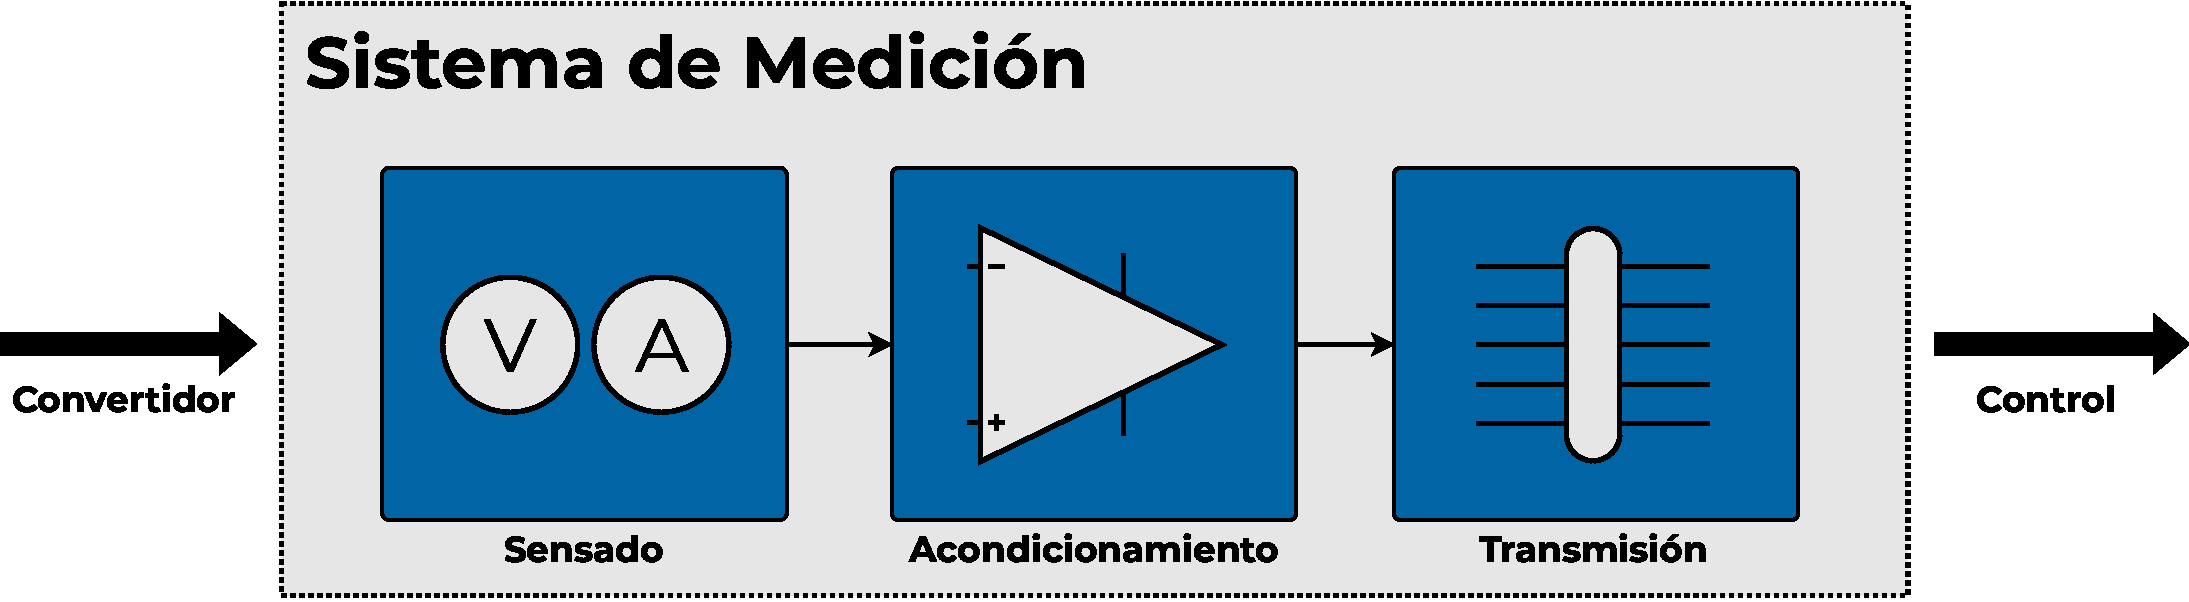
\includegraphics[scale=0.4]{Imagenes/Sistema Medicion.pdf}
    \caption{Sistema de medición de la plataforma, con las tres etapas que lo conforman.}
    \label{diag_medicion}
\end{figure}

Este sistema comienza con la adquisición de los parámetros de interés provenientes del convertidor, tarea llevada a cabo por los sensores de tensión y corriente que conforman la {\Medium etapa de sensado}. Sin embargo, estos datos obtenidos no se presentan en una forma que nuestro sistema de control sea capaz de procesar, por lo que se necesita la siguiente etapa del sistema, la {\Medium etapa de acondicionamiento}, que se encarga de adecuar los datos obtenidos por los sensores para que puedan ser utilizados por el controlador. Finalmente, necesitamos una forma de llevar estos datos desde el sistema de medición hasta el controlador, función que es llevada a cabo por el último bloque de la figura, la {\Medium etapa de transmisión}.\\

Vamos a tratar el diseño de este sistema en el orden que se observa en la figura, por lo que se comenzará por la etapa de sensado o adquisición de datos.\\

\subsubsection{Etapa de Sensado}

En este sistema, los únicos parámetros a medir son tensiones y corrientes, tanto de la pila de combustible a la entrada como de la carga variable a la salida. Previamente a la seleccion de los sensores a utilizar, vamos a realizar una breve categorización y explicación de los métodos de sensado disponibles para ambos parámetros, comenzando por las tensiones.\\

\paragraph{Tecnologías de Sensado de Tensión}

Este es el más simple de los dos casos, ya que los sistemas de control ya trabajan con señales expresadas en tensiones, por lo que no es requerido ningún tipo de transductor, únicamente una adaptación de niveles que es llevada a cabo por la etapa de acondicionamiento. Por esta razón, lo único necesario en este caso es la obtención directa de la tensión buscada, siempre minimizando la perturbación que esta medición introduce al sistema.\\

\paragraph{Tecnologías de Sensado de Corriente}

A diferencia del caso de las tensiones, para poder obtener una medición de corriente se debe realizar algún tipo de transducción que transforme la información de corriente en valores de tensión que puedan ser utilizados por el sistema de control. Existen múltiples tecnologías de sensado y transucción de corriente fundamentalmente distintas, cada una con sus propias características, ventajas y desventajas. Vamos a dedicar algunos párrafos a su clasificación y descripción.\\

\subparagraph{Resistencia Shunt}

Es el método conceptualmente más sencillo de todos, y consiste en interponer al camino de la corriente un resistor \textit{shunt} $R_S$, es decir una resistencia de muy bajo valor (generalmente en las decenas y unidades de \unit{\milli\ohm}), y luego medir la caída de tensión en el mismo. Esta corriente se encuentra directamente relacionada con la tensión mediante la Ley de Ohm, que luego de reordenar resulta:

\begin{equation}\label{ec_shunt}
    I=\frac{1}{R_S}V_S
\end{equation}

Entonces, con este método se obtiene una relación {\Medium perfectamente lineal} entre entre la tensión medida directamente y la corriente que se quiere obtener, siendo el inverso del valor del resistor (o su conductancia) la constante de proporcionalidad. Al tener la Ley de Ohm como su principio de funcionamiento, este método es capaz de medir todo tipo de corrientes, tanto continua (CC) como alterna (CA). Además, al necesitar únicamente una resistor, es {\Medium sumamente sencillo} de implementar.\\

Sin embargo, al estar circulando toda la corriente a través del resistor, se genera una {\Medium pérdida de energía significativa}, ya que la potencia disipada depende del cuadrado de la corriente. Si tomamos la plataforma como ejemplo, donde la corriente de pila $i_{FC}$ en el primario puede llegar a un máximo de \SI[]{10}[]{\ampere}, una resistencia shunt de \SI[]{50}[]{\milli\ohm} puede llegar a disipar una potencia de \SI[]{5}[]{\watt}. Por esta razón, este método no es factible para mediciones de grandes corrientes.\\

La precisión de este método también se {\Medium deteriora con la frecuencia}, ya que para frecuencias suficientemente altas, los efectos de la inductancia parásita $L_S$ y el efecto skin generan un aumento de la impedancia que afecta a la medición.\\

Dadas las altas potencias que puede llegar a disipar un resistor shunt, la temperatura puede presentar un problema si su coeficiente de temperatura no es adecuado. Los fabricantes de estas resistencias tienen esto en cuenta y fabrican los componentes con materiales de bajo coeficiente de temperatura.\\

\begin{figure}[h]
    \centering
    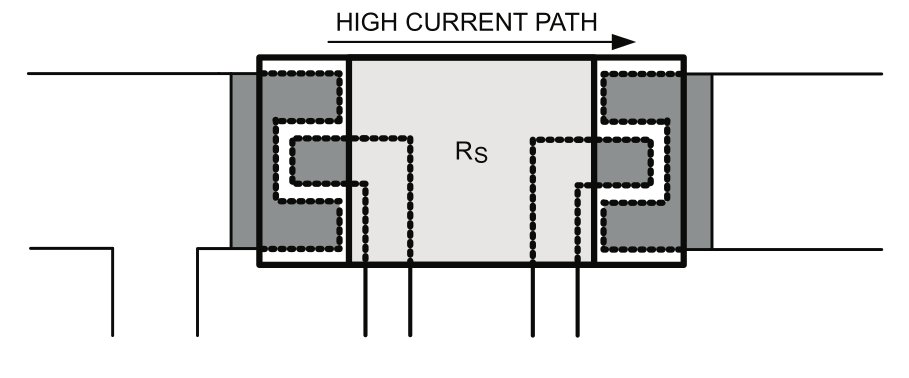
\includegraphics[scale=1.1]{Imagenes/Conexion Kelvin.png}
    \caption{Conexión Kelvin de cuatro cables para el sensado de corriente con un resistor shunt de montaje superficial.}
    \label{conexion_kelvin}
\end{figure}

Sin embargo, esto no puede solucionar el error introducido por el coeficiente de temperatura de las soldaduras, que se exacerban particularmente para valores bajos de resistencia. Para solventarlo, se debe utilizar la conexión de cuatro cables o Kelvin, que separa el camino de alta corriente de las conexiones de sensado, como se ve en la figura \ref{conexion_kelvin}.\textsuperscript{\cite{CurrentSensing}}\\

\subparagraph{Bobina de Rogowski}

Este es un método de medición de corriente basado en la Ley de Inducción de Faraday, y por lo tanto, {\Medium provee aislamiento eléctrico} por su propio principio funcionamiento, a diferencia del método anterior. Este dispositivo consiste, fundamentalmente, en una bobina de forma toroidal y núcleo no ferromagnético a través de la cual se hace pasar el conductor del que se quiere medir la corriente.\\

\begin{figure}[h]
    \centering
    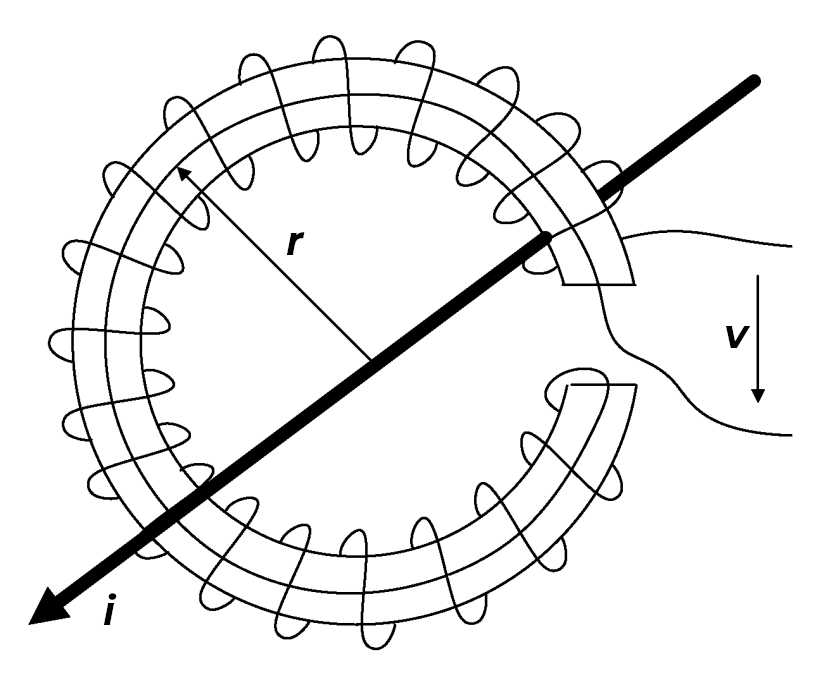
\includegraphics[scale=0.2]{Imagenes/Bobina Rogowski.png}
    \caption{Esquema de una bobina de Rogowski utilizada para medir la corriente $i$ que circula por el conductor.}
    \label{bobina_rogowski}
\end{figure}

Utilizando las leyes de Ampere (que relaciona la integral de un campo magnético en un camino cerrado con la corriente que este encierra) y Faraday (que relaciona la velocidad de cambio de un flujo magnético con la tensión o fuerza electromotriz) se puede obtener una expresión para la tensión medida en bornes de la bobina en función de la corriente de interés. Siguiendo el desarrollo de \cite{CurrentSensing}, se obtiene la siguiente expresión para la tensión de salida.

\begin{equation*}
    v = -\frac{NA\mu_0}{2\pi r}\cdot \frac{di}{dt}
\end{equation*}

Donde $N$ es la cantidad de vueltas de la bobina, $A$ es el área de un corte de la bobina, y $r$ es el radio de la bobina. Sin embargo, en esta ecuación la tensión de salida depende de la velocidad de cambio de la corriente que nos interesa. Entonces, se debe agregar un integrador de constante de integración $k$ a la salida de la bobina, para obtener la tensión $v_o$ dependiente de la corriente que nos interesa.

\begin{equation}\label{ec_rogowski}
    v_o = -k\cdot\frac{NA\mu_0}{2\pi r}\cdot i + v_o(0)
\end{equation}

Una gran ventaja de esta tecnología, es que al no utilizar un núcleo ferromagnético, tiene un rango de medición {\Medium altamente lineal}, comparable con el de una medición por shunt. Además de esto, al no tener que conectar nada al circuito en estudio, prácticamente {\Medium no introduce perturbaciones}, existiendo únicamente pequeños efectos causados por la inductancia de la bobina.\\

Comparado con el resistor shunt, este método presenta muy {\Medium bajas pérdidas} energéticas, al no tener circulación de altas corrientes. Por esta razón, este método es capaz de medir muy {\Medium grandes corrientes}, del orden de los \unit{\mega\ampere}, presentando una clara ventaja respecto al shunt.\\

Sin embargo, al estar su funcionamiento basado en la detección de un cambio de flujo magnético, este sensor es {\Medium incapaz de detectar corrientes continuas}, y tiene dificultades con la detección de componentes de baja frecuencia (es común la utilización de estas bobinas en conjunto con otros sensores capaces de detectar continua).\\

Otra desventaja que dificulta su implementación para nuestra aplicación, es que estas bobinas {\Medium ocupan un gran espacio} y no resulta sencillo integrarlas de forma compacta en una placa de circuito impreso. Además, por esto y por la necesidad de implementar un integrador, su costo es considerable frente al shunt.\\

\subparagraph{Transformador de Corriente}

Al igual que la bobina de Rogowski, este método se aprovecha de los principios establecidos por la ley de inducción de Faraday, por lo que también tiene {\Medium aislación intrínseca}. Su construcción es similar a las bobinas, con una vuelta de bobinado en el primario y una gran cantidad de vueltas en el secundario, pero a diferencia de estas, tiene un núcleo de material ferromagnético. Luego, conectada al secundario se encuentra una resistencia de sensado $R_S$ por la que circula la corriente de secundario $i_s$, generando una caída de tensión $v_s$. Se mide esta tensión, al igual que en el caso del shunt, y se obtiene la corriente del primario en función de esta.

\begin{equation*}
    i = Ni_s + \frac{N}{L_m}\int_t v_s\cdot dt
\end{equation*}

Donde $N$ es la cantidad de vueltas del transformador y $L_m$ es la inductancia magnetizante del transformador. Si reemplazamos la corriente del secundario $i_s$ por la expresión del shunt de la ecuación \ref{ec_shunt}, obtenemos la expresión de la corriente en función de la tensión medida.

\begin{equation}\label{ec_trafocorriente}
    i = N\frac{v_s}{R_S} + \frac{N}{L_m}\int_t v_s\cdot dt
\end{equation}

El término integral de esta ecuación indica que este método es {\Medium incapaz de medir corrientes continuas}: si la corriente $i$ del primario contiene componentes de CC, la corriente magnetizante aumenta hasta que todo el componente de corriente circula únicamente por la inductancia magnetizante $L_m$.\\

Como las vueltas $N$ del secundario pueden ser muy elevadas, se puede obtener una corriente de secundario muy baja, y en consecuencia unas {\Medium bajas pérdidas de energía}. Además, si el término integrador es pequeño (que es el caso para altas frecuencias), las corrientes de primario y secundario son prácticamente proporcionales, resultando en un sensor con {\Medium buena linealidad}.\\

\begin{figure}[h]
    \centering
    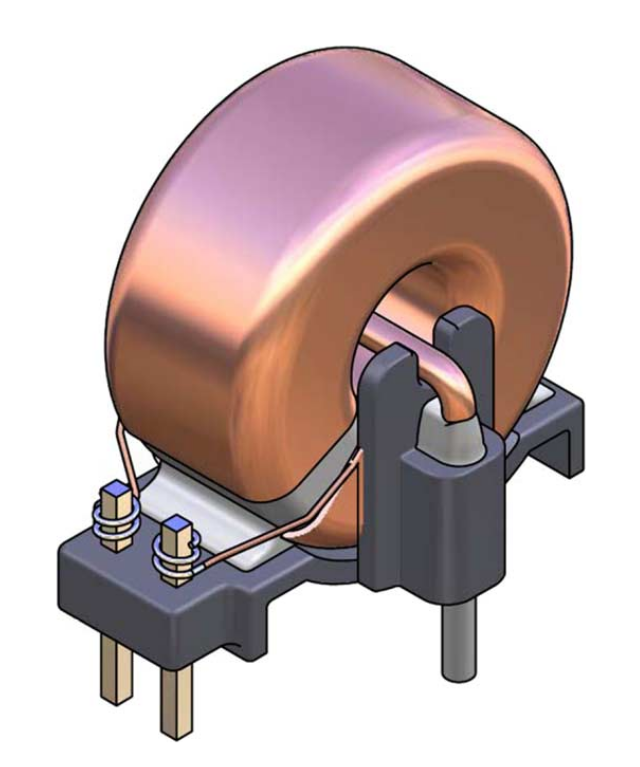
\includegraphics[scale=0.2]{Imagenes/Trafo Corriente.png}
    \caption{Transformador de corriente con una vuelta de primario y múltiples vueltas de secundario.}
    \label{trafo_corriente}
\end{figure}

La inductancia $L_m$ introduce errores de medición, ya que la corriente que circula por ella no circula por la resistencia de sensado, y por lo tanto esto disminuye la caída de tensión $v_s$. Este es un fenómeno conocido como \textit{droop}, y se exacerba particularmente para pulsos de corriente de tiempos largos de encendido en el primario (esto es de interés para nuestra aplicación, dados los pulsos generados por la conmutación de las llaves).\\

Además, como se ve en la figura \ref{trafo_corriente}, su integración en una plaqueta puede ser problemático por su {\Medium gran tamaño}. Sin embargo, hoy en día son muy populares en aplicaciones de convertidores, dado su {\Medium bajo costo} y su salida que suele ser directamente compatible con conversores analógico-digitales.\\

\subparagraph{Efecto Hall}

Finalmente, una tecnología que se utiliza mucho hoy en día son los sensores por efecto Hall, del tipo de medición de campo magnético, basados en el efecto homónimo descubierto por Edwin Hall en 1879. Este efecto consiste en una fina placa metálica sobre la que circula una corriente $I$, atravesada perpendicularmente por un campo magnético $B$, genera una diferencia de potencial $v$ perpendicular a ambos.

\begin{figure}[h]
    \centering
    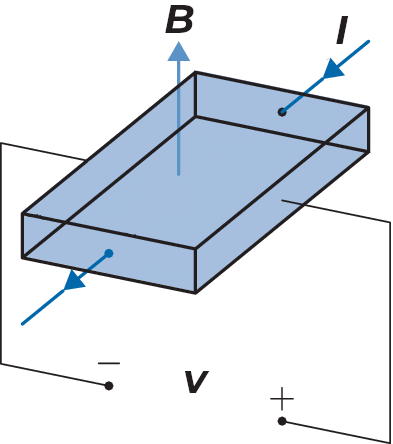
\includegraphics[scale=0.35]{Imagenes/Efecto Hall.png}
    \caption{Diagrama que muestra el principio de funcionamiento de un sensor de corriente por efecto Hall.}
    \label{efecto_hall}
\end{figure}

Entonces, generando un campo magnético que atraviese una placa por la que circula la corriente de interés $i$, se puede medir la tensión que cae en ellas y obtener por medio de esta el valor de la corriente según la ecuación de Hall.

\begin{equation}
    I = v\cdot\frac{nqd}{B}
\end{equation}

Dónde $q$ es la carga de los portadores, $n$ la densidad de portadores y $d$ el grosor de la placa. Como $n$ y $q$ son parámetros que dependen exclusivamente del material utilizado, se suelen consolidar en un parámetro llamado coeficiente de Hall $R_H$, que se define como la inversa del producto de $n$ y $q$. Entonces, la ecuación del sensor resulta:

\begin{equation}\label{ec_hall}
    I = v\cdot\frac{d}{R_HB}
\end{equation}

Como se puede ver por la ecuación, este método posee una {\Medium buena linealidad}, y además, como la corriente circula por un simple conductor, la perturbación introducida es mínima y tiene {\Medium bajas pérdidas de potencia}.\\

Al igual que los métodos de bobina de Rogowski y transformador de corriente, este método, por su principio de funcionamiento, ya {\Medium incluye aislación galvánica}. Pero, a diferencia de los otros métodos magnéticos e inductivos, los sensores de efecto Hall son perfectamente {\Medium capaces de realizar mediciones de corriente continua}.\\

En tanto a sus problemas, los materiales utilizados para las placas metálicas de los sensores suelen tener {\Medium elevadas constantes de temperatura}, por lo que pueden resultar muy susceptibles a cambios de temperatura por sobrecalentamiento. También, para un campo magnético nulo existe una tensión de salida de \textit{offset} no nula, por lo que se requiere electrónica adicional para compensar por este error.\\

Sin embargo, hoy en día existen soluciones integradas en pequeños empaquetados de montaje superficial como los SOIC o SOP, que incluyen un sensor de efecto hall con toda la electrónica asociada necesaria para compensar la tensión de offset y las variaciones por temperatura. Estas son soluciones compactas y de alta precisión, a pesar de su precio mayor comparado con otros métodos.\\\pagebreak

\subparagraph{Resumen}

A modo de resumen de todo lo explicado, se presenta la tabla \ref{tabla:resumen_sensores} que contiene las principales características de interés de las tecnologías de medición de corriente explicadas.\\

\setlength{\tabcolsep}{6pt}
\renewcommand{\arraystretch}{1.5}
\begin{table}[h]
\begin{center}
    \begin{tabular}{l|lllll}
         & {\SemiBold Ancho de Banda} & {\SemiBold Precisión} & \makecell[l]{{\SemiBold Medición} \\ {\SemiBold de CC}} & {\SemiBold Aislación} & {\SemiBold Pérdidas}\\
        \hline
        Shunt & \unit{\kilo\hertz}-\unit{\mega\hertz} & \num{0,1}\% - \num{2}\% & Sí & No & \unit{\milli\watt}-\unit{\watt}\\
        \makecell[l]{Bobina de \\ Rogowski} & \unit{\kilo\hertz}-\unit{\mega\hertz} & \num{0,1}\% - \num{1}\% & No & Sí & \unit{\milli\watt}\\
        Transformador & \unit{\kilo\hertz}-\unit{\mega\hertz} & \num{0,1}\% - \num{1}\% & No & Sí & \unit{\milli\watt}\\
        Efecto Hall & \unit{\kilo\hertz} & \num{0.5}\% - \num{5}\% & Sí & Sí & \unit{\milli\watt}
    \end{tabular}
    \caption{Resumen de las características principales de cada tecnología de sensado de corriente.\textsuperscript{\cite{CurrentSensing}}}
    \label{tabla:resumen_sensores}
\end{center}
\end{table}

Con la información de los distintos tipos de sensores de corriente que se explicaron, se deben seleccionar los modelos de los sensores de la tecnología adecuada para la medición de las variables, buscando en catálogos de sensores.\\

\paragraph{Sensor de Corriente $\mathbf{i_o}$}

La corriente de salida $i_o$ es la variable a medir más importante, ya que es la que directamente controla la potencia de salida que se entrega al bus de continua del sistema híbrido. Por esta razón, debe cumplir algunos requerimientos que se enumeran a continuación.\\

\begin{itemize}
    \item Capacidad de corriente mayor a \SI[]{4.5}[]{\ampere}.
    \item Tensión de operación mayor a \SI[]{100}[]{\volt}.
    \item Precisión de medición debajo del $\pm$1\%.
    \item Ancho de banda $BW$ por encima de \SI[]{40}[]{\kilo\hertz}, el doble de la frecuencia de conmutación.
    \item Capacidad de medir componentes de CC.
    \item Es deseable que el sensor esté galvánicamente aislado del circuito del convertidor.\\
\end{itemize}

La necesidad de medir componentes de corriente continua elimina automáticamente la posibilidad de usar una bobina de Rogowski o un transformador de corriente. Por lo tanto, nos quedan como opciones únicamente la resistencia shunt y el sensor de efecto Hall, que dado que ambos son capaces de precisiones debajo del \num{1}\% y anchos de banda de \unit{\kilo\hertz}, se decide utilizar un {\Medium sensor de efecto Hall}, por la presencia de aislación galvánica.\\

Entonces, buscando sensores de corriente de efecto Hall en catálogos online, se llegó al modelo {\Medium TMCS1100A4} de Texas Instruments, un sensor Hall de medición bidireccional (corrientes positivas y negativas) de alta precisión y aislamiento básico, todo en un encapsulado de montaje superficial de ocho pines tipo SOIC-8. Según la hoja de datos del fabricante, este dispostivo esta pensado para ser utilizado en la medición de corrientes de inversores y puentes completos. Sus especificaciones se presentan en la tabla \ref{tabla:sensor_hall}.\\

\setlength{\tabcolsep}{6pt}
\renewcommand{\arraystretch}{1.5}
\begin{table}[H]
\begin{center}
    \begin{tabular}{llrrrrr}
    {\SemiBold Fabricante} & {\SemiBold Modelo} & $\mathbf{I_{in}}$ [\unit{\ampere}] & $\mathbf{V_{in}}$ [\unit{\volt}] & $\mathbf{BW}$ [\unit{\kilo\hertz}] & $\mathbf{e_i}$ & {\SemiBold Sens.} [\unit{\milli\volt\per\ampere}]\\
    \hline
    \makecell[l]{Texas \\ Instruments} & TMCS1100A4 & \num{12} & \num{600} &  \num{80} & $\pm$\num{0.9}\% & \num{400}
    \end{tabular}
    \caption{Especificaciones del sensor de corriente por efecto Hall, modelo TMCS1100A4 de Texas Instruments.\textsuperscript{\cite{TMCS1100}}}
    \label{tabla:sensor_hall}
\end{center}
\end{table}

Dónde $I_{in}$ es la máxima corriente unidireccional medible, $V_{in}$ es la máxima tensión de operación en la entrada, $BW$ es el ancho de banda de la medición, y $e_i$ es la precisión o error relativo de la medición.\\ 

La variante A4 tiene una sensibilidad de \SI[]{400}[]{\milli\volt\per\ampere}, poniendo la tensión de salida en el rango de \num{0} a \SI[]{1.8}[]{\volt} para una corriente de salida $i_o$ máxima de \SI[]{4.5}[]{\ampere}. Además, si tomamos el error relativo máximo de $\pm$\num{0.9}\%, se obtiene que la precisión absoluta es de $\pm$\SI[]{40}[]{\milli\ampere}, más que suficiente para ser aplicado en la plataforma.\\

\begin{figure}[h]
    \centering
    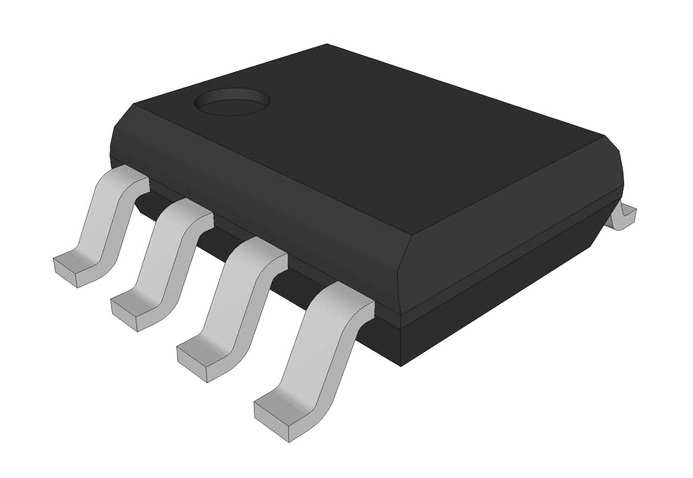
\includegraphics[scale=0.8]{Imagenes/SOIC8.jpg}
    \caption{Sensor de corriente por efecto Hall, modelo TMCS1100A4 de Texas Instruments, en su encapsulado tipo SOIC-8.}
    \label{encapsulado_hall}
\end{figure}

El sensor tiene cuatro pines para el sensado de corriente, dos llamados IN+ y dos llamados IN-. Como se trata de medición de corriente, se debe conectar el sensor en serie al camino de corriente, con la corriente entrando por los pines IN+ y saliendo por los pines IN-.\\

Luego, el pin de tensión de referencia VREF se conecta a masa, ya que de esta manera se configura el sensor para utilizar un rango de medición unidireccional\textsuperscript{\cite{TMCS1100}}, ya que en nuestro caso la corriente solo puede circular hacia la carga (para obtener un rango bidireccional, se alimentar el pin con una tensión igual a la mitad de la alimentación).\\

\begin{figure}[h]
    \centering
    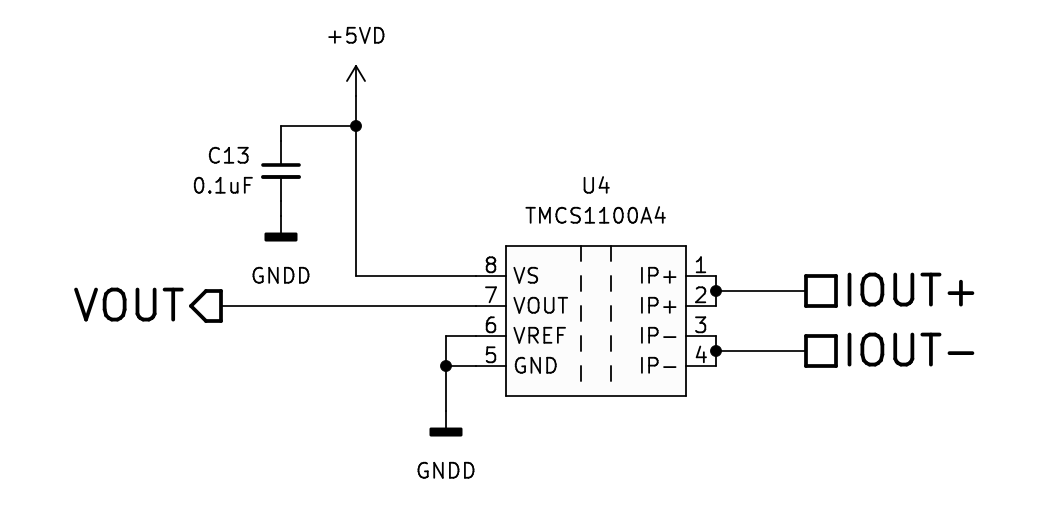
\includegraphics[scale=1]{Imagenes/Conexion TMCS1100.png}
    \caption{Conexión del sensor TMCS1100A4, según recomendaciones del fabricante.}
    \label{conexion_TMCS1100}
\end{figure}

Todas las conexiones a tierra del sensor se realizan en la tierra de señal o digital $GND_D$, ya que se encuentran todas del segundo lado del dispositivo, aislados del circuito de potencia del convertidor. El pin VS se conecta a la alimentación digital del sistema requiriendo una tensión de \SI[]{5}[]{\volt} positivos, con un capacitor de filtro conectado en derivación según recomendación del fabricante.\\

El pin de salida VOUT, como se verá mas adelante, se debe conectar primero a un circuito que acondicione la señal que el sensor arroja, para luego poder ser conectado a la entrada del conversor analógico-digital (ADC) del controlador que convertirá los datos analógicos de corriente en datos digitales que pueda procesar.\\

\paragraph{Sensor de $\mathbf{v_{FC}}$, $\mathbf{i_{FC}}$ y $\mathbf{v_o}$}

Por una cuestión de simplicidad, se eligió buscar una única solución integrada que sea capaz de medir múltiples variables, en nuestro caso una corriente y dos tensiones. Dado que las variables restantes son de menor importancia, limitar el requerimiento de ancho de banda respecto a la corriente de salida. A continuación se detallan algunos requerimientos.\\

\begin{itemize}
    \item Capacidad de medición de corriente por arriba de \SI[]{10.5}[]{\ampere}.
    \item Capacidad de medición de tensión por arriba de \SI[]{75}[]{\volt}.
    \item Precisión mejor o igual al $\pm$\num{2}\%.
    \item Capacidad de medir componentes de CC.
    \item Ancho de banda $BW$ lo más alto posible.
    \item Es deseable que el sensor esté galvánicamente aislado del circuito del convertidor.\\
\end{itemize}

Buscando en catálogos online de distintos fabricantes se encontró el {\Medium circuito integrado LM5056A} de Texas Instruments, descrito por el fabricante como un \quotes{Dispositivo de Administración de Potencia de Sistemas de Alta Tensión}.\\

Consiste en un sensor de corriente de tipo shunt, junto con un sensor de tensión a la entrada del shunt y una medición de tensión auxiliar, con la capacidad adicional de calcular la potencia en base a las mediciones.  Al usar medición de tipo shunt, tiene la capacidad de medir componentes de CC, pero no posee aislación galvánica. Se detallan algunas especificaciones a continuación.\\

\setlength{\tabcolsep}{6pt}
\renewcommand{\arraystretch}{1.5}
\begin{table}[H]
\begin{center}
    \begin{tabular}{llrrrrr}
    {\SemiBold Fabricante} & {\SemiBold Modelo} & $\mathbf{V_{in/out}}$ [\unit{\volt}] & $\mathbf{f_m}$ [\unit{\kilo\hertz}] & $\mathbf{I_{in(FSR)}}$ [\unit{\milli\volt}] & $\mathbf{e_{i}}$ & $\mathbf{e_v}$\\
    \hline
    \makecell[l]{Texas \\ Instruments} & LM5056A & \num{100} & \num{1} &  \num{27}/\num{54.4} & $\pm$\num{1.25}\% & $\pm$\num{1}\%
    \end{tabular}
    \caption{Especificaciones del sensor combinado de tensión, corriente y potencia por shunt, modelo LM5056A de Texas Instruments.\textsuperscript{\cite{LM5056A}}}
    \label{tabla:LM5056A}
\end{center}
\end{table}

Donde $V_{in/out}$ es la máxima tensión de entrada y salida medible, $f_m$ es la frecuencia de muestreo del sensor, $I_{in(FSR)}$ es la tensión de fondo de escala de medición de corriente, $e_i$ es la precisión de la medida de corriente, y $e_v$ es la precisión de la medida de tensión.\\

Los parámetros analógicos de tensión y corriente medidos por el LM5056A son muestreados y convertidos a información digital mediante un conversor analógico-digital interno de \num{12} bits de resolución, (es decir $2^12 = 4096$ niveles distintos) con frecuencia de muestreo $f_m$ de \SI[]{1}[]{\kilo\hertz} como muestra la tabla. Una vez convertidos, se pueden transmitir mediante la interfaz de bus I\textsuperscript{2}C que provee el integrado, con pines SDAO para salida de datos, SDAI para entrada de datos y SCL para entrada de reloj. Esta interfaz se explica más adelante en la sección 3.4.3, sobre la etapa de transmisión.\\



Este dispositivo viene en un empaquetado de montaje superficial del tipo HTSSOP-28 de 28 pines (figura \ref{encapsulado_LM5056}), que también incluye un contacto plano en la parte inferior, de conexión opcional para la disipación de calor.\\

\begin{figure}[h]
    \centering
    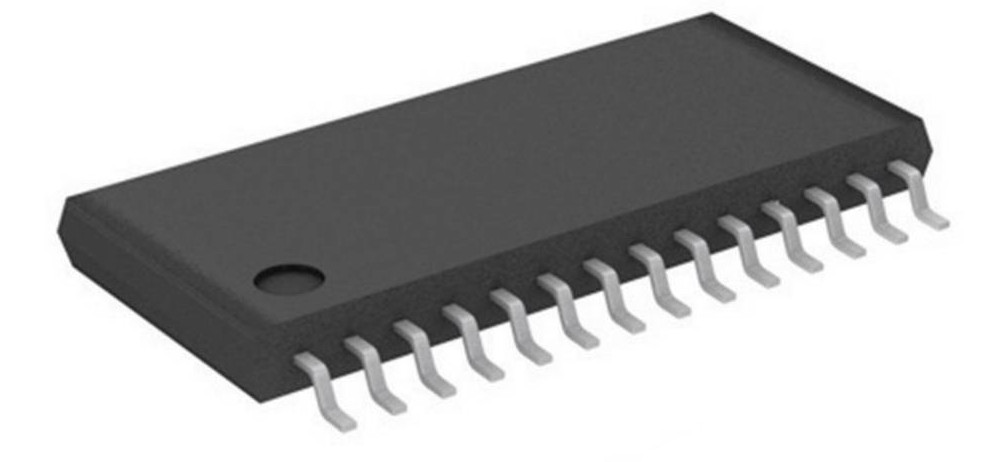
\includegraphics[scale=0.15]{Imagenes/HTSSOP.jpg}
    \caption{Sensor de tensión, corriente y potencia, modelo LM5056A de Texas Instruments, en su encapsulado tipo HTSSOP-28.}
    \label{encapsulado_LM5056}
\end{figure}

\lipsum[1]\\

\begin{figure}[h]
    \centering
    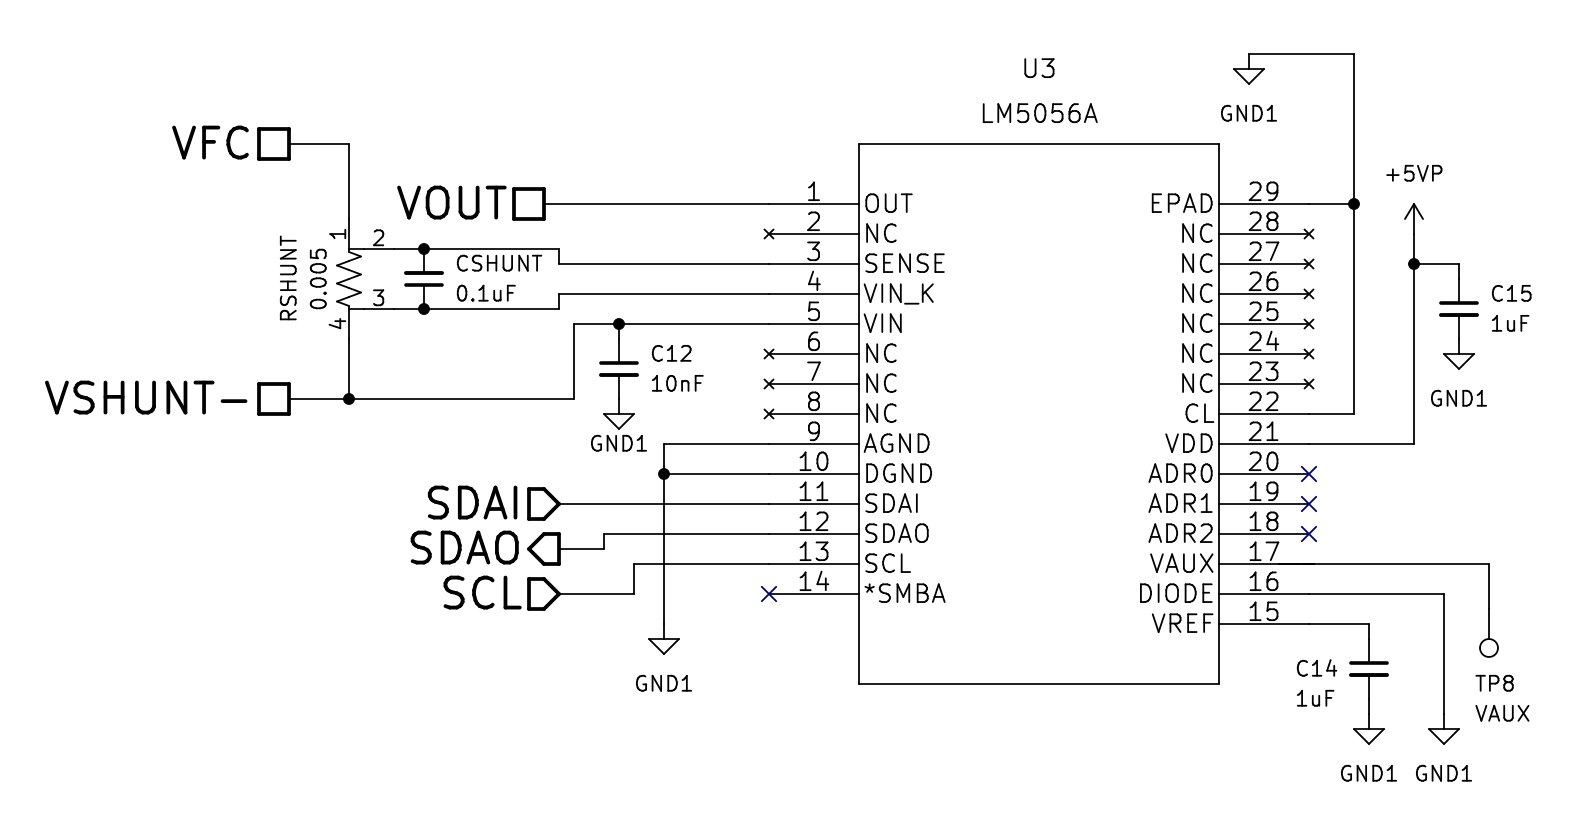
\includegraphics[scale=1]{Imagenes/Conexion LM5056A.png}
    \caption{Conexión del sensor LM5056A para medir tensión y corriente de entrada y tensión de salida, según especificaciones del fabricante.}
    \label{conexion_LM5056}
\end{figure}

\lipsum[2]\\

\subsubsection{Etapa de Acondicionamiento}

\lipsum[1]\\

\subsubsection{Etapa de Transmisión}

\lipsum[2]\\

\lipsum[3]\\